\documentclass[10pt]{report}

\usepackage{enumerate} % for enumerate counter
\usepackage{subcaption} % for subfigures
\usepackage{amsthm} % for QED
\usepackage{mathtools} % for delimiter

\usepackage{listings} % for code
\lstset{ 
	language=R,
	basicstyle=\footnotesize\ttfamily,
	numbers=none,
	stepnumber=1,
	numbersep=8pt,
	showspaces=false,
	showstringspaces=false,
	showtabs=false,
	frame=single,
	tabsize=2,
	captionpos=t,
	breaklines=true,
	breakatwhitespace=false
} 

\usepackage{float} % for figure [H]
\usepackage{booktabs} % for tabular
\usepackage{caption} % for \caption*
\usepackage[export]{adjustbox} % for valign=t
\usepackage{array} % for column type m
\usepackage{verbatim}
\usepackage{graphicx}
%\graphicspath{ {imgs/} }
\usepackage{fancyhdr}
\usepackage{amssymb}
\usepackage{amsmath}

%%%%%%Pagination
\setlength{\topmargin}{-.3 in}
\setlength{\oddsidemargin}{0in}
\setlength{\evensidemargin}{0in}
\setlength{\textheight}{9.in}
\setlength{\textwidth}{6.5in}

%Cover
\newcommand{\hwTitle}{Homework \#4}
\newcommand{\hwCourse}{Applied Statistics}
\newcommand{\hmClassInstructor}{Professor Lulu Kang}

\title{
	\vspace{2in}
	\textmd{\textbf{\hwCourse\\\hwTitle}}\\
	\vspace{0.3in}\large{\textit{\hmClassInstructor}}
	\vspace{3in}
}
\author{\textbf{Zhihao Ai}}
\date{}

%Header
\pagestyle{fancy}
\fancyhead[L]{Zhihao Ai}
\fancyhead[C]{Math 484}
\fancyhead[R]{Homework 4}
%%%%%%

%Global settings
%\everymath{\displaystyle}
\setlength\parindent{0pt}

%Custom commands
\newcommand{\ds}{\displaystyle}
\newcommand{\ts}{\textstyle}

\newcolumntype{N}{>$ c <$}
\newcolumntype{M}[1]{>{\centering\arraybackslash $}m{#1}<{$}}

\newcommand{\abs}[1] {\left| #1 \right|}

\DeclarePairedDelimiter\autoparen{(}{)}
\newcommand{\pa}[1]{\autoparen*{#1}}

\newcommand{\var} {\text{var}}

\newcommand{\m}[1] {\mathbf{#1}}

\begin{document}

\maketitle

\section*{Problem 1}
(Ex. 7.19) Refer to \textbf{Commercial properties}  Problem 6.18.
\begin{enumerate}[a.]
	\item 
	Transform the variables by means of the correlation transformation (7.44) and fit the standardized regression model (7.45).
	
	By solving $\m{b} = \m{r}^{-1}_{XX} \m{r}^{}_{YX}$, we have
	\[
	\m{b} = [-0.5478526, 0.4236468, 0.04846136, 0.5027571]'
	\]
	So the standardized regression model is $Y^*_i = -0.5478526 X^*_{i1} + 0.4236468 X^*_{i2} + 0.04846136 X^*_{i3} + 0.5027571 X^*_{i4}$.
	
	\item 
	Interpret the standardized regression coefficient $b^*_2$.
	
	With other predictor variables fixed, the rental rates ($Y$) will increase by 0.4236468 standard deviations if operating expenses and taxes ($X_2$) increase by 1 standard deviation.
	
	\item 
	Transform the estimated standardized regression coefficients by means of (7.53) back to the ones for the fitted regression model in the original variables. Verify that they are the same as the ones obtained in Problem 6.18c.
	
	Employing the relations
	\begin{align*}
		b_k &= \pa{\frac{s_Y}{s_k}} b^*_k \quad (k=1,\dots,p-1)\\
		b_0 &= \bar{Y} - b_1 \bar{X}_1 - \dots - b_{p-1} \bar{X}_{p-1}
	\end{align*}
	We have
	\[
	\m{b} = [1.220059\mathrm{e}+01, -1.420336\mathrm{e}-01, 2.820165\mathrm{e}-01, 6.193435\mathrm{e}-01, 7.924302\mathrm{e}-06]'
	\]
	which is the same as the one ontained in Problem 6.18c.
\end{enumerate}

\section*{Problem 2}
(Ex. 7.24) Refer to \textbf{Brand preference}  Problem 6.5.
\begin{enumerate}[a.]
	\item 
	Fit first-order simple linear regression model (2.1) for relating brand liking ($Y$) to moisture content ($X_1$). State the fitted regression function.
	
	Fitting the model for relating $Y$ to $X_1$, we have
	\lstinputlisting{p2/24a.txt}
	So the fitted regression function is $\hat{Y} = 50.775 + 4.425 x_1$.
	
	\item 
	Compare the estimated regression coefficient for moisture content obtained in part (a) with the corresponding coefficient obtained in Problem 6.5b. What do you find?
	
	The fitted regression function in Problem 6.5b is $\hat{Y} = 37.65 + 4.425 x_1 + 4.375 x_2$. The $b_1$ coefficients are the same.
	
	\item 
	Does $SSR(X_1)$ equal $SSR(X_1|X_2)$ here? If not, is the difference substantial?
	
	Yes, they both equal 1566.45.
	
	\item 
	Refer to the correlation matrix obtained in Problem 6.5a. What bearing does this have on your findings in parts (b) and (c)?
	
	The correlation between $X_1$ and $X_2$ is 0, meaning the two predictor variables are uncorrelated. When they are uncorrelated, the effects ascribed to them by a first-order regression model are the same no matter which other of the variables are included in the model, so the corresponding coefficients in parts (b) are the same. Likewise, the marginal contribution of one variable in reducing the error sum of squares when the other variable is in the model is the same as when it is in the model alone, hence $SSR(X_1) = SSR(X_1|X_2)$.
	
\end{enumerate}

\section*{Problem 3}
(Ex. 8.24) \textbf{Assessed valuations}
\begin{enumerate}[a.]
	\item 
	Plot the sample data for the two populations as a symbolic scatter plot. Does the regression relation appear to be the same for the two populations?
	
	Below is the symbolic scatter plot:
	\begin{figure}[H]
		\centering
		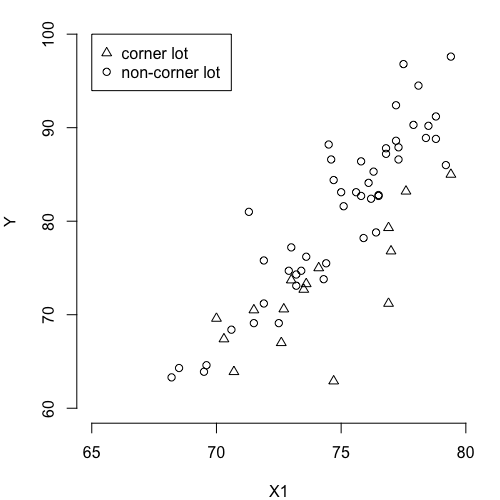
\includegraphics[width=.5\linewidth]{p3/24a.png}
	\end{figure}
	The regression relation does not appear to be the same.
	
	\item 
	Test for identity of the regression functions for dwellings on corner lots and dwellings in the other locations; control the risk of Type I error at .05. State the alternatives, decision rule, and conclusion.
	
	The tentative model is given by
	\[
	Y_i = \beta_0 + \beta_1 X_{i1} + \beta_2 X_{i2} + \beta_3 X_{i1}X_{i2} + \epsilon_i
	\]
	where
	\begin{align*}
		X_{i1} &= \text{assessed valuation}\\
		X_{i2} &=
		\begin{cases}
		0 & \text{if on non-corner lots}\\
		1 & \text{if on corner lots}
		\end{cases}
	\end{align*}
	The alternatives are
	\begin{align*}
		H_0: &\ \beta_2 = \beta_3 = 0\\
		H_a: &\ \text{not both $\beta_2 = 0$ and $\beta_3 = 0$}
	\end{align*}
	The test statistic is:
	\[
	F^* = \frac{MSR(X_2, X_1 X_2 | X_1)}{MSE} = \frac{SSR(X_2 | X_1) + SSR(X_1 X_2 | X_1, X_2)}{2} \div MSE
	\]
	The decision rule is
	\begin{align*}
	\text{If } F^* \le F(0.95; 2, 60) = 3.150411, \text{ conclude } H_0\\
	\text{If } F^* > F(0.95; 2, 60) = 3.150411, \text{ conclude } H_a
	\end{align*}
	\lstinputlisting{p3/24b.txt}
	Using the results above, $F^* = (453.1+113.0)/2/15.2 = 18.62171 > 3.150411$. So we conclude $H_a$, that the regression functions for the two dwellings locations are not identical.
	
	\item 
	Plot the estimated regression functions for the two populations and describe the nature of the differences between them.
	\begin{figure}[H]
		\centering
		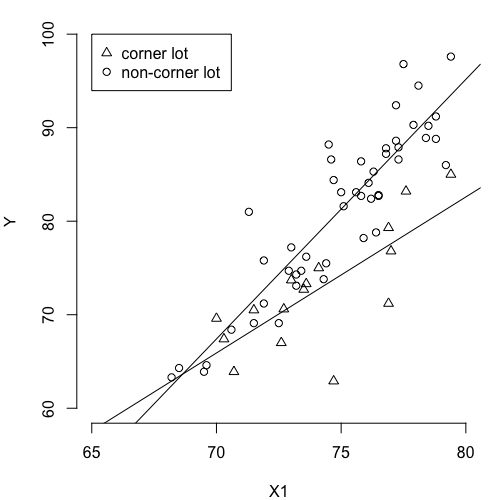
\includegraphics[width=.5\linewidth]{p3/24c.png}
	\end{figure}
	The response functions are:
	\begin{align*}
		E(Y) &= \beta_0 + \beta_1 X_1 + \beta_2(0) + \beta_3(0) = \beta_0 + \beta_1 X_1 \quad \text{non-corner lots}\\
		E(Y) &= \beta_0 + \beta_1 X_1 + \beta_2(1) + \beta_3(X_1) = (\beta_0 + \beta_2) + (\beta_1 + \beta_3) X_1 \quad \text{corner lots}
	\end{align*}
	$\beta_2$ here indicated how much greater is the $Y$ intercept of the response function for the class coded 1 than that for the class coded 0. $\beta_3$ indicates how much smaller is the slope of the response function for the class coded 1 than that for the class coded 0. The nature of the differences is the effect of the class and the interaction of $X_1$ and $X_2$ on the regression.
\end{enumerate}

\end{document}

